\documentclass{beamer}
\usepackage[UTF8,space,hyperref]{ctex}
\usepackage{graphicx} % ⋯⋯导言区其他内容
\usepackage{subfigure} 
\usepackage{caption}
\usepackage{amsmath}
\usepackage{cite}

\usepackage[numbers,sort&compress]{natbib} %压缩参考文献标号
\setbeamertemplate{caption}[numbered]
\newcommand{\upcite}[1]{\textsuperscript{\textsuperscript{\cite{#1}}}} %参考文献上标
\captionsetup{font={scriptsize}}  %图片注释字体大小
\usetheme{Frankfurt}
\author{齐家兴}
\title{基于多样性数据生成和集成学习的两类非平衡大数据分类}
\institute {\large河北大学数学与信息科学学院}

\begin{document}

%目录设置,每一章都显示目录并加粗
\AtBeginSection[] { 
  \begin{frame}
    \frametitle{目录} 
    \tableofcontents[currentsection,hideothersubsections] 
  \end{frame} 
  \addtocounter{framenumber}{-1}  %目录页不计算页码
}

\begin{frame}
    \titlepage
    \begin{flushright}
        指导老师:翟俊海
    \end{flushright}
\end{frame}

\begin{frame}{目录}
    \tableofcontents
\end{frame}

\section{课题来源及研究的目的和意义}
\begin{frame}{课题来源}\pause
    目前,对不平衡数据分类问题的研究是非常活跃的研究领域,根据Guo等\upcite{haixiang2017learning}统计,在过去的10年内,总计192个期刊和会议共发表527篇关于非平衡问题的论文。这证明迄今为止,非平衡问题还是一个非常有价值的研究课题。
    
\end{frame}

\begin{frame}{课题来源}\pause
        \begin{columns}
            \column{0.5\textwidth}
            \begin{minipage}[c][0.4\textheight][c]{\linewidth}
                \centering
                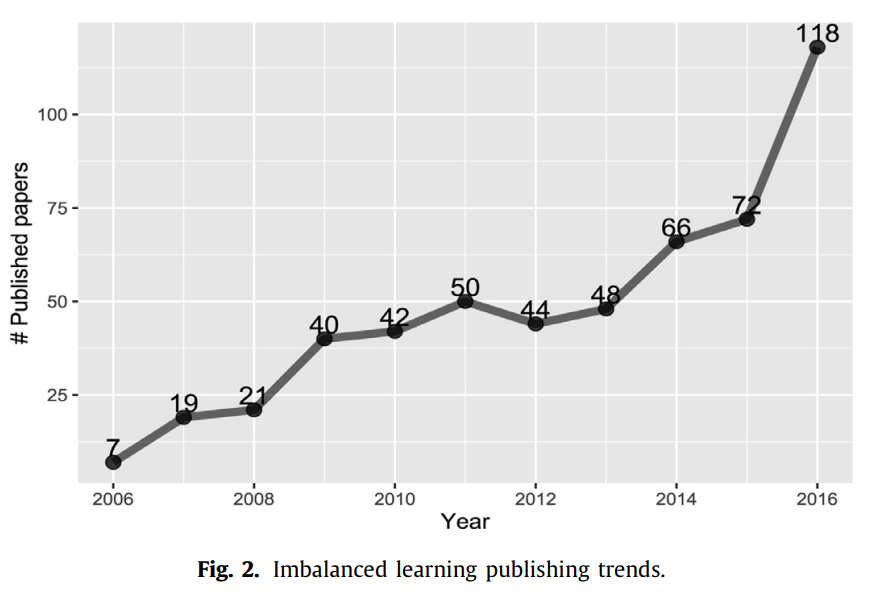
\includegraphics[scale=0.2]{trend.png}
            \end{minipage}

            \begin{minipage}[c][0.4\textheight][c]{\linewidth}
                \centering
                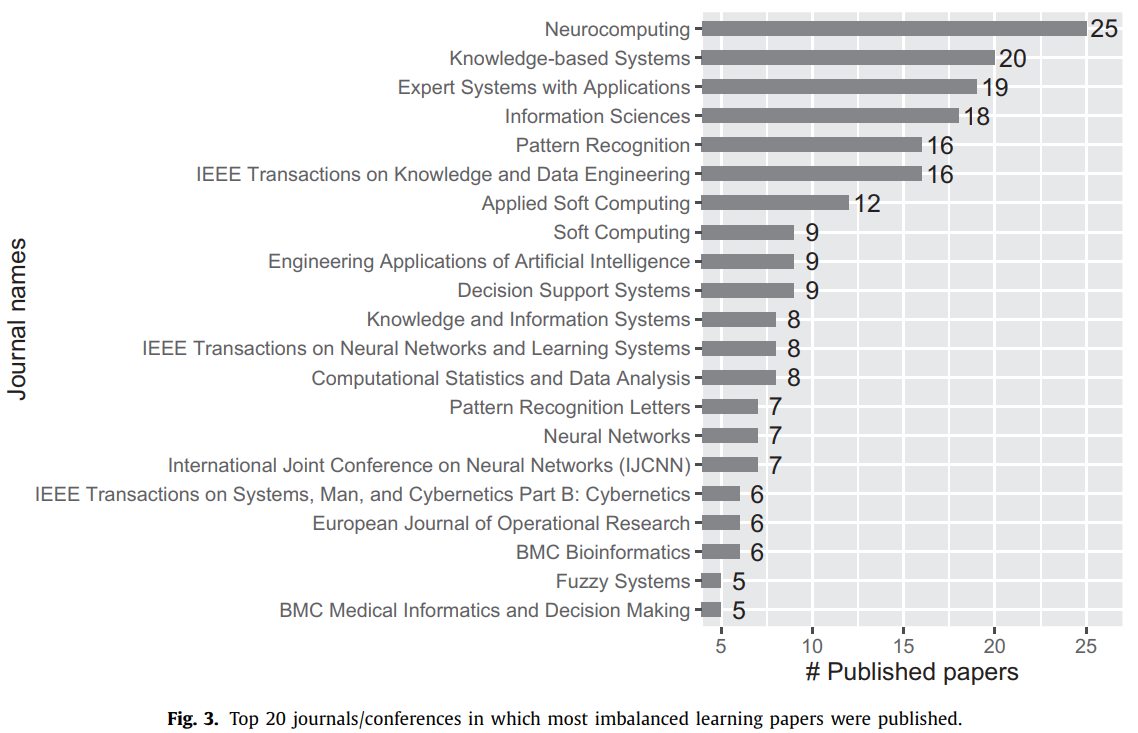
\includegraphics[scale=0.2]{top20.png}
            \end{minipage}
            
            \column{0.5\textwidth} % remember add this to the other clumn
            \begin{minipage}[c][0.4\textheight][c]{\linewidth}
                \begin{itemize}
                    \item 2006年至2016年,关于非平衡问题论文发表情况。
                \end{itemize}
                
            \end{minipage}

            \begin{minipage}[c][0.4\textheight][c]{\linewidth}
                \begin{itemize}
                    \item 关于非平衡问题,发表论文数TOP20期刊或会议
                \end{itemize}
                
            \end{minipage}
        \end{columns}
\end{frame}

\begin{frame}{研究目的和意义}\pause
    \begin{itemize}
        \item 非平衡问题分类如下两种\upcite{haixiang2017learning}:
        \begin{itemize}
            \item 两类非平衡问题 
            \item 多类非平衡问题
        \end{itemize}
    \end{itemize}
\end{frame}

\begin{frame}{研究目的和意义}\pause
    \begin{block}{两类非平衡问题:}
        即数据中某一类别的样例数远远小于另一类别,并且把数量比较多的样本称为多数类样本(负类样本),数量较少的样本称为少数类样本(正类样本)\upcite{wang2012multiclass,he2008learning,van2009knowledge}
    \end{block}
    目前研究人员提出了许多方法解决二类不平衡问题。其中,对数据集进行重采样,增加少数类样例数目或者减少多数类样例数目,使数据集平衡化,就是一种非常有效的方法。
\end{frame}


\begin{frame}{研究目的和意义}\pause
    Gracia等\upcite{garcia2012effectiveness}分析了不同采样算法对分类性能的影响,实验表明上采样的结果往往比下采样要好,因为下采样可能会丢失一些重要的信息。
\end{frame}



\begin{frame}{研究目的和意义}\pause
    目前,大多数上采样方法,会导致原始数据集类别分布的改变,有可能导致分类器在训练过程中出现过拟合的情况。另外,在某些情况下,大多数上采样方法缺乏可解释性,并且效果有限。因此,研究一种可解释性强且有效的数据上采样方法是非常必要的。
\end{frame}



\section{国内外研究现状}
\begin{frame}{国内外研究现状}\pause
    目前,对于数据对于类别不平衡问题,已有的文献中已经提出了不同的解决方法。主要分为以下三类\upcite{spelmen2018review}:
    \begin{itemize}
        \item 数据层面
        \item 算法层面
        \item 混合的方法
    \end{itemize}    
\end{frame}

\begin{frame}{国内外研究现状}\pause
    \noindent数据层面:\\
    主要通过样本重采样技术对数据集预处理,有以下三种方法:
    \begin{itemize}
        \item 上采样
        \item 下采样
        \item 两者结合
    \end{itemize}
\end{frame}

\begin{frame}{国内外研究现状}\pause
    \noindent上采样:\\
    \begin{itemize}
        \item 
        1998年,Ling等\upcite{ling1998data}出了随机上采样。
        \item 
        2002年,Chawla等\upcite{chawla2002smote}提出了少数类生成上采样方法SMOTE
        \item  
        2005年,HAN等\upcite{han2005borderline}提出了Borderline-SMOTE
        \item  
        2015年,S等\upcite{saez2015smote}提出SMOTE-IPF
        \item  
        其它基于SMOTE的改进方法\upcite{hu2009msmote, ali2019imbalance}
    \end{itemize}
    
\end{frame}

\begin{frame}{国内外研究现状}\pause
    \noindent下采样:\\
    \begin{itemize}
        \item  
        1972年,Wilson等\upcite{wilson1972asymptotic}提出ENN
        \item 
        1997 Kubat等\upcite{kubat1997addressing}提出One-sided Selection
        \item 
        1998年,Ling等\upcite{ling1998data}出了随机下采样。
        \item 
        2016年,Ha等\upcite{ha2016new}提出了基于遗传算法的下采样方法GAUS 
    \end{itemize}
    
\end{frame}

\begin{frame}{国内外研究现状}\pause
    随着深度学习及神经网络的发展,神经网络在许多任务场景中都能起到良好的效果,越来越多的研究人员投入到这一领域当中。因此利用神经网络或者深度学习技术解决非平衡问题,近几年也有许多的研究成果。
    \begin{itemize}
        \item 
        Ryota等\upcite{shimizu2018balanced}利用平衡mini-batch方法,用于解决工业产品视觉质量检测问题。
        \item 
        Cenggoro等\upcite{cenggoro2018deep}提出了一种类专家的生成对抗模型CE-GAN,作为不平衡分类的解决方案。
        \item  
        Zhou等\upcite{zhou2018gan}通过改进SSGAN模型,用于生成少数类样本。
        \item 
        Chen\upcite{Chen2018CGAN}集成GMM和CGAN,提出一种GMM-CGAN模型用作数据增强。
    \end{itemize}
    
    
\end{frame}



\section{主要研究内容及创新点}
\begin{frame}{主要研究内容及创新点}\pause
    传统上采样方法(如SMOTE系列),生成的数据在一些情况下缺乏可解释性,会导致生成的数据没有意义,给训练分类器增加了难度。并且当数据或者维度较多时,计算量比较大甚至无法运行。
\end{frame}

\begin{frame}{主要研究内容及创新点}\pause
    
    \begin{figure}[t]
        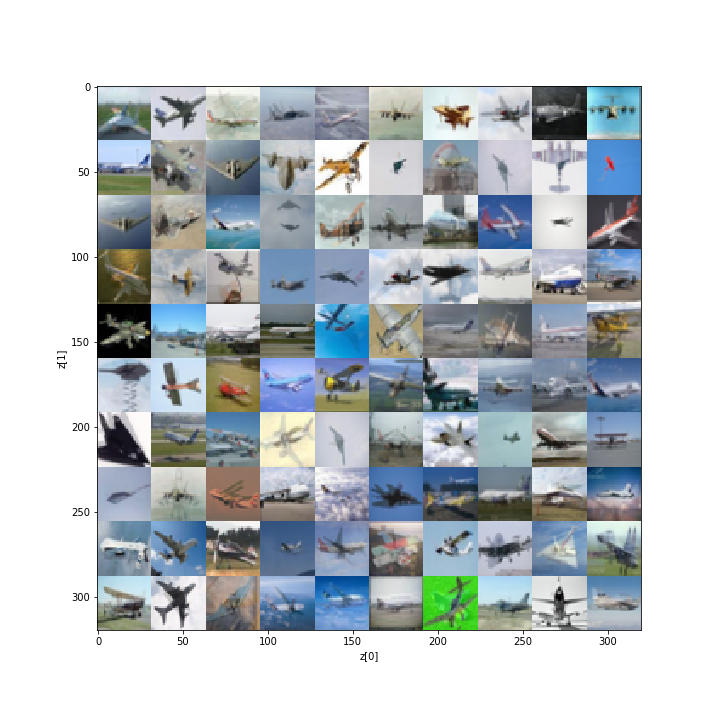
\includegraphics[scale=0.25]{zeros9.png}
        \caption{ SMOTE对Cifar10上采样}
    \end{figure}
\end{frame}

\begin{frame}{主要研究内容及创新点}\pause
    \begin{figure}[t]
        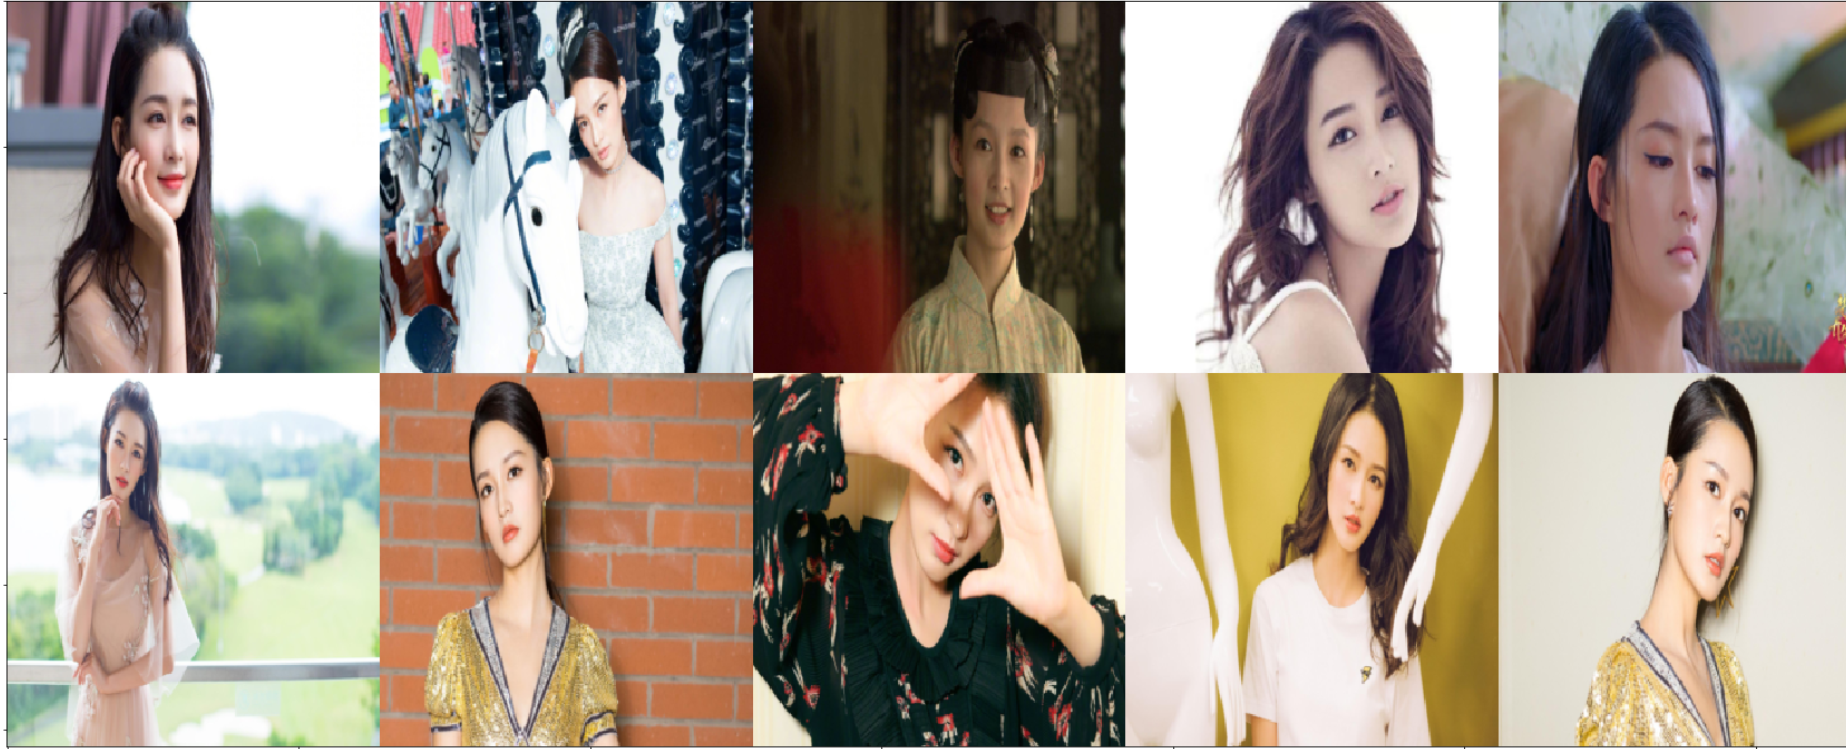
\includegraphics[scale=0.2]{liTrue.png}
        \caption{原始图像}
    \end{figure}
\end{frame}


\begin{frame}{主要研究内容及创新点}\pause
    \begin{figure}[t]
        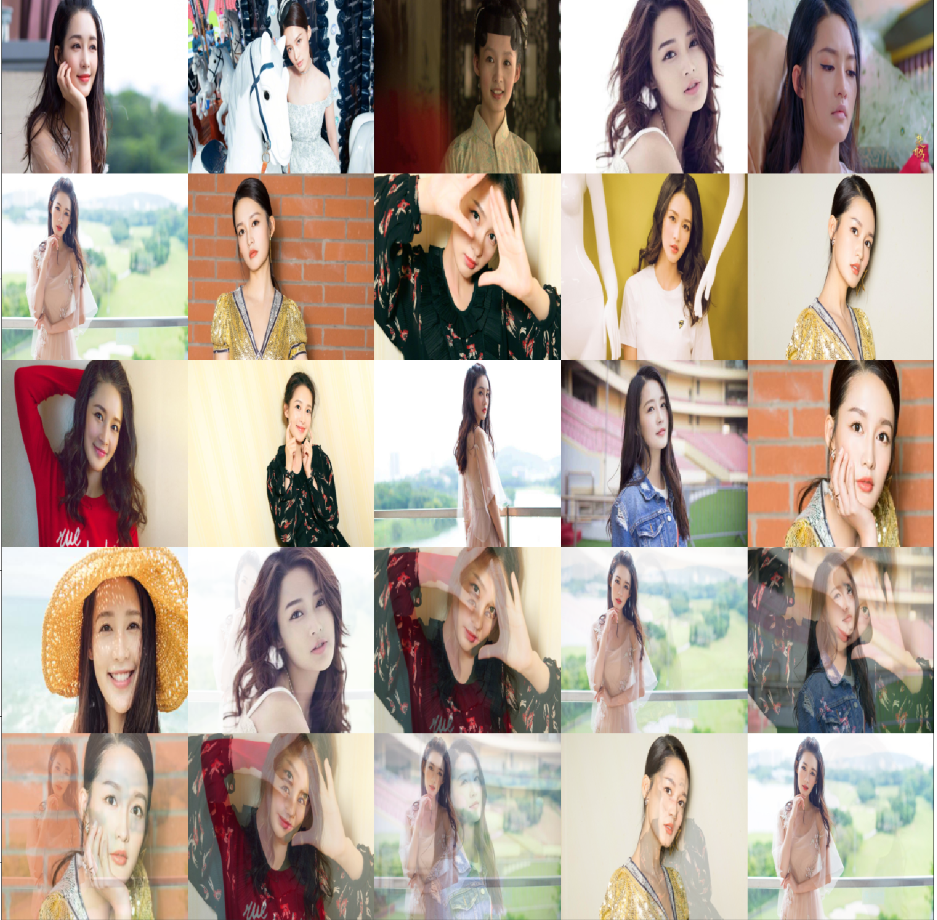
\includegraphics[scale=0.25]{liSMOTE1.png}
        \caption{上采样后的图像}
    \end{figure}
\end{frame}

\begin{frame}{主要研究内容及创新点}\pause
    \begin{figure}[t]
        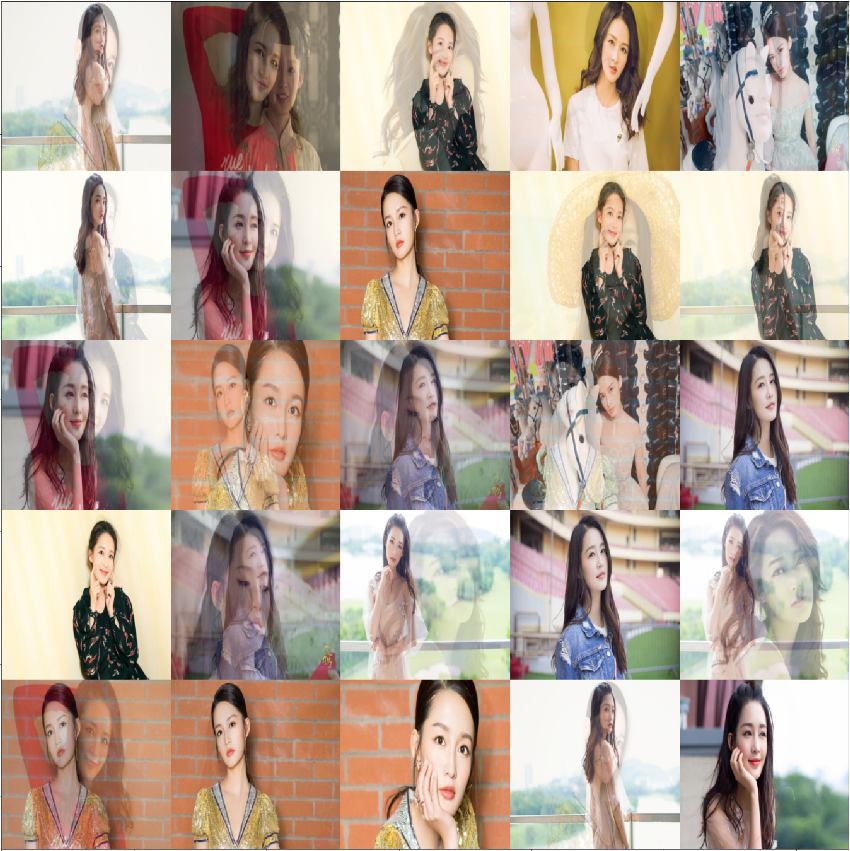
\includegraphics[scale=0.25]{liSMOTE2.png}
        \caption{上采样后的图像}
    \end{figure}
\end{frame}

\begin{frame}{主要研究内容1}\pause
    针对这种情况,我们通过生成对抗网络或者变分自编码器,并设计相应的网络结构,训练生成模型用于生成有意义的少数类样本。
\end{frame}

\begin{frame}{主要研究内容2}\pause
    在对少数类样本进行上采样的过程中,已有的样本采样方法不能保证生成样本的多样性,导致生成的样本和已有的样本过于相似,不能增加有效的信息。为了保证生成样本的多样性,本论文拟采用一个指标(如类内散度最大化)来评价生成样本的多样性,并指导样本的生成。从而可以有效的扩充少数类样本,增加有效的数据信息。
\end{frame}

\begin{frame}{主要研究内容3}\pause
    为了保证不过多的对少数类样本上采样,导致数据的冗余。我们将多数类样本划分为K个子集,令每个子集与上采样后的少数类样本构成一个相对平衡数据集,以减少上采样的数量。但是由于K的取值对于不同数据集来说可能不同,所以对K的选取需要讨论、实验,找到合适的取值。
\end{frame}

\begin{frame}{主要研究内容4}\pause
    将多数样本划分为K个子集后,各个子集与上采样后的少数类样本构成一个相对平衡的数据集,但是我们无法知道当平衡比例达到多少时就可以有效的训练分类器。针对这一问题,决定研究数据集在不同平衡比例下分类器性能的变化,找到一个合适的平衡比例。
\end{frame}

\begin{frame}{创新点}\pause
    \begin{itemize}
        \item 基于生成对抗网络或者变分自编码器对两类不平衡大数据进行数据生成
        \item 通过集成的方法减少少数类样例上采样的数量,并提高分类器的性能
        \item 采用一种多样性评价指标,从而可以有效的增加数据信息,改善分类的效果
    \end{itemize}
\end{frame}



\section{研究方案及进度安排}
\begin{frame}{研究方案及进度安排}\pause
    \begin{itemize}
        \item 
        通过阅读大量的文献和资料,掌握生成对抗网络、变分自编码器以及集成算法的原理和实现方式。
        \item 
        选择合适的模型结构,以及训练方式
        \item 
        选择实验数据集
        \item 
        实验分析,通过实验结果对所提出的方法进行分析,并与已有的上采样方法比较。
        \item 
        在导师的指导下,撰写毕业论文。
    \end{itemize}
\end{frame}

\section{研究过程中可能遇到的困难以及解决措施}

\begin{frame}[c]\frametitle{研究目前存在的一些问题(非确定性)}
    由于深度学习领域目前有很多的不确定性,基于此可能会对我们的研究造成一些的困扰。
    \begin{itemize}
        \item 论文中提出的算法与开源的代码实现不匹配
        \item 良好的算法实现与不良的代码实现之间有着巨大差距
        \item 训练的随机性,即训练相同的模型两次能否获得相同的分数是十分重要的,
        由于某些GPU操作存在随机性,如果禁用这些操作就会造成时间的损失
    \end{itemize}
\end{frame}

\begin{frame}{研究过程中可能遇到的困难以及解决措施}\pause
    遇到的困难:
    \begin{itemize}
       \item 
       模型的选择以及实验的设计,评价指标的选择。
       \item 
       在没有得到其它方法开源实现的情况下,如何能够保证实验结果正确性,以及比较的公平性。
    \end{itemize}
\end{frame}

\begin{frame}[allowframebreaks]\frametitle{参考文献}
    \scriptsize
    \bibliographystyle{gbt7714-2005}
    \bibliography{ref}
\end{frame}

\end{document}